\documentclass[11pt]{article}

% Packages
\usepackage[margin=1in]{geometry}
\usepackage{amsmath, amssymb}
\usepackage{graphicx}
\usepackage{caption}
\usepackage{subcaption}
\usepackage{enumitem}
\usepackage{hyperref}
\usepackage{fancyhdr}
\usepackage{titlesec}
\usepackage{xcolor}
% \usepackage{subfigure}
\usepackage{float}
\usepackage{graphicx}
\usepackage{subcaption}

% Header/Footer
\pagestyle{fancy}
\fancyhf{}
\rhead{ML Project Report}
\lhead{Jonas Gericke and Yexuan Wang}
\cfoot{\thepage}

% Section formatting
\titleformat{\section}{\large\bfseries}{\thesection}{1em}{}
\titleformat{\subsection}{\normalsize\bfseries}{\thesubsection}{1em}{}

% Title
\title{\textbf{Efficient Algorithms for Lasso Regression}}
\author{Jonas Gericke and Yexuan Wang \\
Applied Machine Learning in Python -- LMU Munich \\
\texttt{jonas.gericke@campus.lmu.de and yexuan.wang@campus.lmu.de}}
\date{July 9, 2025}

\begin{document}


\maketitle

\section{Task Overview}

This project focuses on solving Lasso regression using two optimization methods: SubGradient Descent and ISTA. The goal is to compare their performance in terms of convergence speed, sparsity, and sensitivity to initialization and hyperparameters.
Through this project, we aim to understand how different algorithms behave when solving sparse regression problems.
We ran experiments to compare SubGradient Descent and ISTA on Lasso regression. Tests include synthetic data, different initializations, varying \(\lambda\) and learning rates, and a real-world case on the Boston Housing dataset.

\section{Methods}

We compare two methods for solving the Lasso regression problem: SubGradient Descent and Proximal Gradient Descent (ISTA).
SubGradient Descent is simple and widely applicable, but it typically converges slowly and may not effectively promote sparsity. In contrast, ISTA uses proximal updates with soft-thresholding, which leads to faster convergence and sparser solutions. Comparing these two methods highlights the trade-off between simplicity and optimization efficiency in Lasso regression.

\noindent\textbf{The Lasso objective is defined as:}
\[
    \min_{\mathbf{w} \in \mathbb{R}^d} \left\{ \frac{1}{2n} \|\mathbf{Xw} - \mathbf{y}\|_2^2 + \lambda \|\mathbf{w}\|_1 \right\}
\]

\noindent\textbf{SubGradient Descent update:}
\[
    \mathbf{w}^{(t+1)} = \mathbf{w}^{(t)} - \frac{\eta}{n} \left( \mathbf{X}^T ( \mathbf{X} \mathbf{w}^{(t)} - \mathbf{y}) + \lambda \cdot \text{sign}(\mathbf{w}^{(t)}) \right)
\]

\noindent\textbf{ISTA update:}
\[
    \mathbf{w}^{(t+1)} = \text{prox}_{\eta \lambda} \left( \mathbf{w}^{(t)} - \eta \nabla g(\mathbf{w}^{(t)}) \right)
\]
\[
    g(\textbf{w}) = \frac{1}{2n} \| \textbf{X} \textbf{w} - \textbf{y} \|_2^2
\]
\[
    \text{prox}_{\eta \lambda}(z_j) = \text{sign}(z_j) \cdot \max\left( |z_j| - \eta \lambda, \, 0 \right)
\]


\subsection*{Implementation Notes}

We used fixed learning rates and iteration numbers. ISTA is expected to converge faster and yield sparser solutions, which is confirmed in our experiments.

\section{Experiments and Results}


\subsection{Training Loss and Sparsity}
\begin{figure}[H]
    \centering
    \begin{minipage}{0.3\textwidth}
        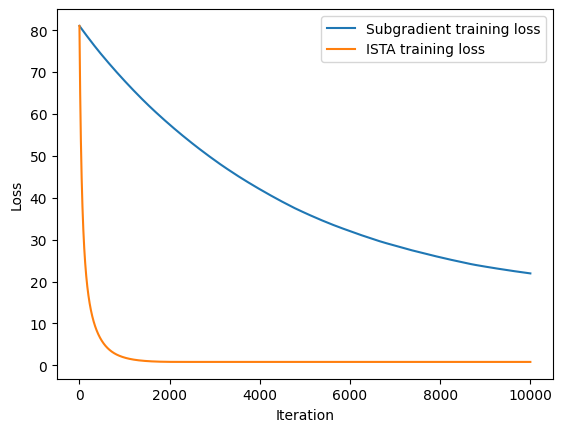
\includegraphics[width=\linewidth]{figures/fig1.png}
    \end{minipage}
    \hfill
    \begin{minipage}{0.5\textwidth}
        \small
        \textbf{Figure 1:} We train Lasso models  on synthetic data with standard normal initialization, \( \lambda = 0.5 \), and learning rate \( 10^{-4} \) for 10,000 epochs. As figure shows,
        ISTA converges much faster than SubGradient Descent and achieves higher sparsity after about 2000 iterations.
    \end{minipage}
\end{figure}


\subsection{Path}
Beyond loss and sparsity metrics, we analyze the evolution of model coefficients during training.
We consider two initialization schemes: random Gaussian and all-zero initialization. With both of initial value, ISTA quickly drives many coefficients to zero, demonstrating strong sparsity-inducing behavior due to its soft-thresholding mechanism. In contrast, SubGradient Descent reduces coefficient magnitudes more slowly.
\begin{figure}[H]
    \centering
    \begin{subfigure}[b]{0.45\textwidth}
        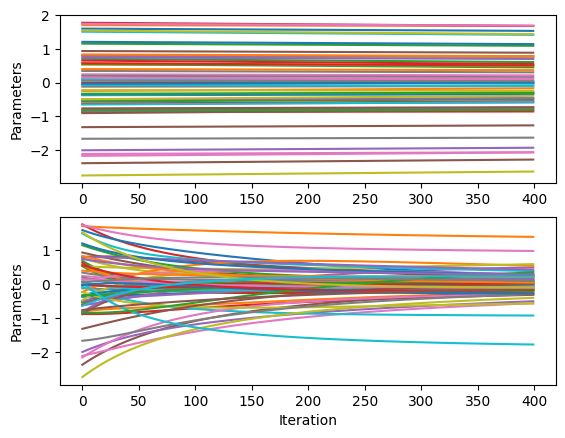
\includegraphics[width=\textwidth]{figures/fig3.png}
        \caption{Initial value starts with random Gaussian}
        \label{fig:sub1}
    \end{subfigure}
    \hfill
    \begin{subfigure}[b]{0.45\textwidth}
        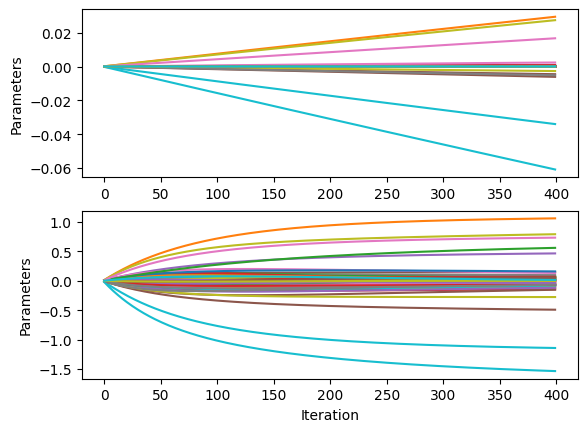
\includegraphics[width=\textwidth]{figures/fig4.png}
        \caption{Initial value starts with 0}
        \label{fig:sub2}
    \end{subfigure}
    %\caption{Comparison under different initializations}
    \label{fig:main}
\end{figure}


%These results further confirm ISTA’s efficiency in promoting sparse solutions under \( \ell_1 \)-regularization.


\subsection{Effect of Different Lambda on Sparsity}

\begin{figure}[H]
    \centering
    \begin{minipage}{0.3\textwidth}
        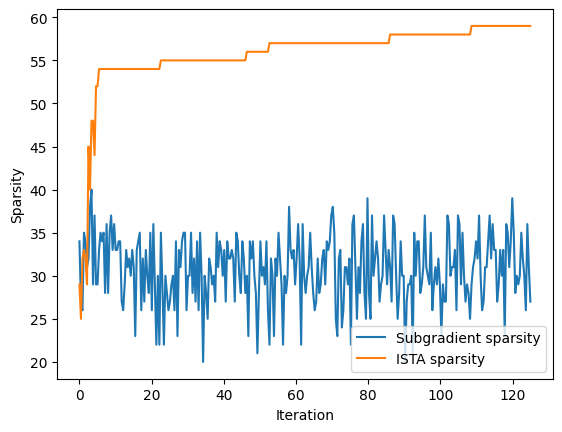
\includegraphics[width=\linewidth]{figures/fig5.png}
    \end{minipage}
    \hfill
    \begin{minipage}{0.5\textwidth}
        \small
        \textbf{Figure 3:}
        The regularization parameter \( \lambda \) controls model sparsity in Lasso. Larger values lead to stronger penalties and sparser solutions.
        ISTA shows a clear increase in sparsity as \( \lambda \) grows, remaining stable and close to maximum sparsity. In contrast, SubGradient Descent fluctuates and maintains lower sparsity, indicating ISTA is more effective at enforcing regularization.
    \end{minipage}
\end{figure}




\subsection{Sensitivity to Initialization}

\begin{figure}[H]
    \centering
    \begin{minipage}{0.3\textwidth}
        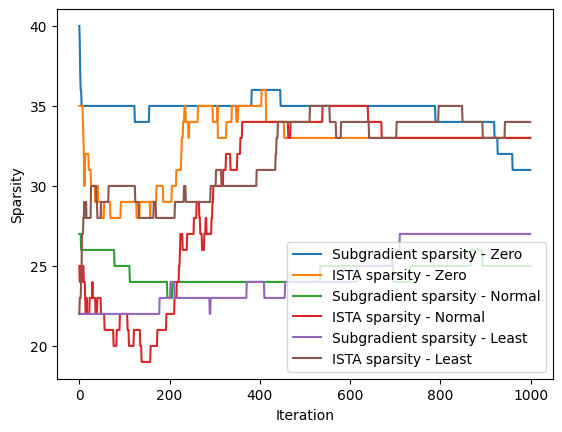
\includegraphics[width=\linewidth]{figures/fig6.png}
    \end{minipage}
    \hfill
    \begin{minipage}{0.5\textwidth}
        \small
        \textbf{Figure 4:}

        Initialization significantly influences the convergence behavior of optimization algorithms. We compare three strategies: zero initialization, random Gaussian initialization, and the least-squares solution \( w_0 = (X^\top X)^{-1} X^\top y \).The results show that ISTA consistently converges to highly sparse solutions regardless of initialization, demonstrating strong robustness. In contrast, SubGradient Descent is more sensitive, especially with random initialization, leading to slower and less stable sparsity patterns.


    \end{minipage}
\end{figure}



\subsection{Convergence with Learning Rate}


\begin{figure}[H]
    \centering
    \begin{minipage}{0.3\textwidth}
        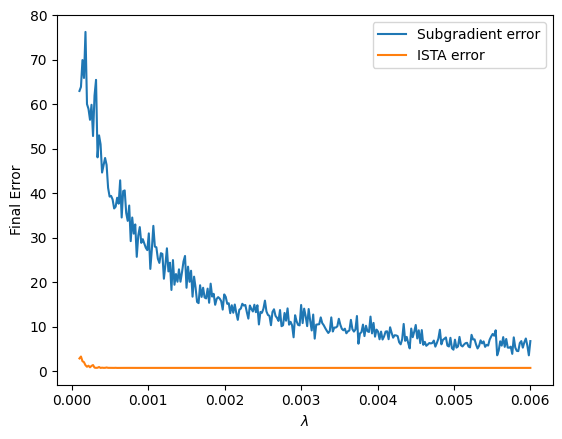
\includegraphics[width=\linewidth]{figures/fig7.png}
    \end{minipage}
    \hfill
    \begin{minipage}{0.5\textwidth}
        \small
        \textbf{Figure 5:}
        To examine the effect of learning rate, we evaluate both SubGradient Descent and ISTA under a range of learning rates from 0.0001 to 0.005.
        As shown in the figure, ISTA exhibits stable and consistently low error across all learning rates, indicating strong robustness to this parameter. In contrast, SubGradient Descent is much more sensitive: at low learning rates it converges slowly with high residual error, and although the error decreases with increasing learning rate, it remains significantly higher than ISTA.
    \end{minipage}
\end{figure}

\subsection{Application to Boston Housing Data}


\begin{figure}[H]
    \centering
    \begin{minipage}{0.3\textwidth}
        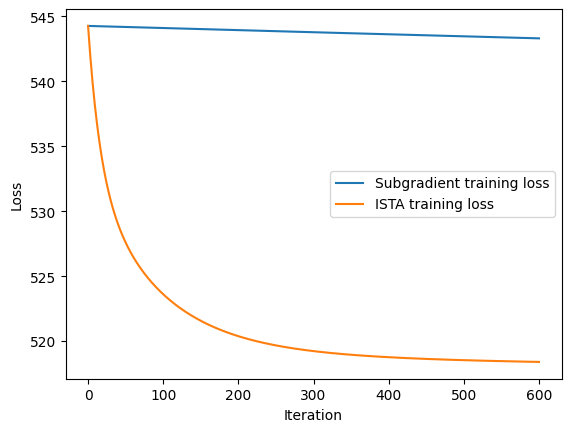
\includegraphics[width=\linewidth]{figures/fig8.png}
    \end{minipage}
    \hfill
    \begin{minipage}{0.5\textwidth}
        \small
        \textbf{Figure 6:}
        Finally, we apply both ISTA and SubGradient Descent to the Boston Housing dataset. The
        target is the median house price.
        As shown in the figure, ISTA achieves much faster convergence in training loss than SubGradient Descent, which aligns with our earlier synthetic results.

    \end{minipage}
\end{figure}


\section{Discussion}

In this project, we investigated and compared two optimization methods for Lasso regression: SubGradient Descent and ISTA.
The key finding is that ISTA consistently outperforms SubGradient Descent in terms of convergence speed and sparsity.
ISTA is more robust to initialization and ISTA handled a wider range of learning rates without becoming unstable, while SubGradient was more sensitive and sometimes required careful tuning.
One limitation of our experiments is that we used a fixed number of iterations for both methods, which might have limited SubGradient Descent’s performance.
For future work, it would be interesting to study accelerated variants like FISTA, compare results on more diverse datasets, and evaluate model performance using cross-validation or test error.





\end{document}



